\documentclass[sigconf]{acmart}

%%
%% \BibTeX command to typeset BibTeX logo in the docs
\AtBeginDocument{%
	\providecommand\BibTeX{{%
			Bib\TeX}}}


%% Rights management information.  This information is sent to you
%% when you complete the rights form.  These commands have SAMPLE
%% values in them; it is your responsibility as an author to replace
%% the commands and values with those provided to you when you
%% complete the rights form.
%\setcopyright{acmlicensed}
%\copyrightyear{2018}
%\acmYear{2018}
%\acmDOI{XXXXXXX.XXXXXXX}
%
%%% These commands are for a PROCEEDINGS abstract or paper.
%\acmConference[Conference acronym 'XX]{Make sure to enter the correct
%	conference title from your rights confirmation emai}{June 03--05,
%	2018}{Woodstock, NY}
%%%
%%  Uncomment \acmBooktitle if the title of the proceedings is different
%%  from ``Proceedings of ...''!
%%
%%\acmBooktitle{Woodstock '18: ACM Symposium on Neural Gaze Detection,
%%  June 03--05, 2018, Woodstock, NY}
%\acmISBN{978-1-4503-XXXX-X/18/06}

\copyrightyear{2024}
\acmYear{2024}
\setcopyright{rightsretained}
\acmConference[CCS '24]{Proceedings of the 2024 ACM SIGSAC Conference on Computer and Communications Security}{October 14--18, 2024}{Salt Lake City, UT, USA}
\acmBooktitle{Proceedings of the 2024 ACM SIGSAC Conference on Computer and Communications Security (CCS '24), October 14--18, 2024, Salt Lake City, UT, USA}
\acmDOI{10.1145/3658644.3670356}
\acmISBN{979-8-4007-0636-3/24/10}

% The following includes the CC license icon appropriate for your paper.
% Download the image from www.scomminc.com/pp/acmsig/4ACM-CC-by-88x31.eps
% and place within your figs or figures folder

\makeatletter
\gdef\@copyrightpermission{
	\begin{minipage}{0.3\columnwidth}
		\href{https://creativecommons.org/licenses/by/4.0/}{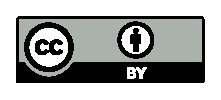
\includegraphics[width=0.90\textwidth]{4ACM-CC-by-88x31.eps}}
	\end{minipage}\hfill
	\begin{minipage}{0.7\columnwidth}
		\href{https://creativecommons.org/licenses/by/4.0/}{This work is licensed under a Creative Commons Attribution International 4.0 License.}
	\end{minipage}
	\vspace{5pt}
}
\makeatother



%%
%% For managing citations, it is recommended to use bibliography
%% files in BibTeX format.
%%
%% You can then either use BibTeX with the ACM-Reference-Format style,
%% or BibLaTeX with the acmnumeric or acmauthoryear sytles, that include
%% support for advanced citation of software artefact from the
%% biblatex-software package, also separately available on CTAN.
%%
%% Look at the sample-*-biblatex.tex files for templates showcasing
%% the biblatex styles.
%%

%%
%% The majority of ACM publications use numbered citations and
%% references.  The command \citestyle{authoryear} switches to the
%% "author year" style.
%%
%% If you are preparing content for an event
%% sponsored by ACM SIGGRAPH, you must use the "author year" style of
%% citations and references.
%% Uncommenting
%% the next command will enable that style.
%%\citestyle{acmauthoryear}


%\usepackage{llncsconf}
%\usepackage{times}
%\usepackage{amsmath,amssymb, amsthm,amsfonts,enumitem,tikz, subcaption, mdframed}
\usepackage{amsmath, amsthm,amsfonts,enumitem,tikz, subcaption, mdframed}
\usepackage{multirow}
%\usepackage{amssymb}
\usepackage{tcolorbox}
\usepackage{comment}
\usepackage{graphicx}
\usepackage{caption}
\usepackage{subcaption}
\usepackage{hyperref}
\usepackage{pgfplots}
\usepackage{booktabs, tabularx}
\usepackage{colortbl}
\usepackage{url}
\usetikzlibrary{arrows,arrows.meta,shapes.arrows, calc, positioning,matrix}


\newtheorem{theorem}{Theorem}[section]
\newtheorem{lemma}{Lemma}[section]
\newtheorem{definition}{Definition}[section]





\begin{document}
	
	%%
	%% The "title" command has an optional parameter,
	%% allowing the author to define a "short title" to be used in page headers.
	\title{Batching-Efficient RAM using Updatable Lookup Arguments}
	%%
	%% The "author" command and its associated commands are used to define
	%% the authors and their affiliations.
	%% Of note is the shared affiliation of the first two authors, and the
	%% "authornote" and "authornotemark" commands
	%% used to denote shared contribution to the research.
	%	\author{Ben Trovato}
	%	\authornote{Both authors contributed equally to this research.}
	%	\email{trovato@corporation.com}
	%	\orcid{1234-5678-9012}
	%	\author{G.K.M. Tobin}
	%	\authornotemark[1]
	%	\email{webmaster@marysville-ohio.com}
	%	\affiliation{%
	%		\institution{Institute for Clarity in Documentation}
	%		\streetaddress{P.O. Box 1212}
	%		\city{Dublin}
	%		\state{Ohio}
	%		\country{USA}
	%		\postcode{43017-6221}
	%	}
	%%
	%% By default, the full list of authors will be used in the page
	%% headers. Often, this list is too long, and will overlap
	%% other information printed in the page headers. This command allows
	%% the author to define a more concise list
	%% of authors' names for this purpose.
	\author{Moumita Dutta}
	\affiliation{
		\institution{Indian Institute of Science}
		\city{Bangalore}
		\country{India}}
	\email{moumitadutta@iisc.ac.in}
	
	\author{Chaya Ganesh}
	\affiliation{
		\institution{Indian Institute of Science}
		\city{Bangalore}
		\country{India}}
	\email{chaya@iisc.ac.in}
	
	\author{Sikhar Patranabis}
	\affiliation{
		\institution{IBM Research India}
		\city{Bangalore}
		\country{India}}
	\email{sikhar.patranabis@ibm.com}
	
	\author{Shubh Prakash}
	\affiliation{
		\institution{Indian Institute of Science}
		\city{Bangalore}
		\country{India}}
	\email{shubhprakash@iisc.ac.in}
	
	\author{Nitin Singh}
	\affiliation{
		\institution{IBM Research India}
		\city{Bangalore}
		\country{India}}
	\email{nitisin1@in.ibm.com}
	
	
	
	
	%	\renewcommand{\shortauthors}{Dutta et al.}
	
	%%
	%% The abstract is a short summary of the work to be presented in the
	%% article.
	\begin{abstract}
		%RAM (random access memory) is a useful primitive in verifiable computation.
		%The RAM primitive allows one to efficiently verify that execution of a program $\mathcal{P}$
		%with read/write access to memory state $\mathsf{st}_0$ results in the final state $\mathsf{st}_1$.
		%The efficiency requires that verification is cheaper than naive execution of $\mathcal{P}$
		%(typically poly-logarithmic) and only requires access to {\em succinct} digests (e.g. Merkle hash) of the state(s).
		%Persistence refers to the fact that state digests allow proving updates to the state across several computations
		%in an incremental fashion.
		
		RAM (random access memory) is an important primitive in verifiable computation.
		In this paper, we focus on realizing RAM with efficient batching property, i.e,
		proving a batch of $m$ updates on a RAM of size $N$ while incurring a cost that is sublinear in $N$.
		Classical approaches based on Merkle-trees or address ordered transcripts to model
		RAM correctness are either concretely inefficient, or incur linear overhead in the size of the RAM.
		Recent works explore cryptographic accumulators based on unknown-order groups (RSA, class-groups)
		to model the RAM state. While recent RSA accumulator based approaches
		offer significant improvement over classical methods,
		they incur linear overhead in the size of the
		accumulated set to compute witnesses, as well as prohibitive constant overheads.
		
		We realize a batching-efficient RAM with superior asymptotic and concrete
		costs as compared to existing approaches. Towards this: (i) we build on recent constructions of lookup arguments to allow efficient
		lookups even in presence of table \textit{updates}, and (ii) we realize a variant of sub-vector relation
		addressed in prior works, which we call {\em committed index lookup}. We combine the two
		building blocks to realize batching-efficient RAM with sublinear dependence on
		size of the RAM. Our construction incurs an amortized proving cost of $\wt{O}(m\log m + \sqrt{mN})$
		for a batch of $m$ updates on a RAM of size $N$.
		Our results also benefit the recent arguments for sub-vector relation, by
		enabling them to be efficient in presence of updates to the table.
		We believe that this is a contribution of independent interest. 
		
		We implement our solution to evaluate its concrete efficiency.
		Our experiments show that it offers significant improvement over existing works on
		batching-efficient accumulators/RAMs, with a substantially reduced resource barrier.
		
	\end{abstract}


		
		
	
	
	%%
	%% The code below is generated by the tool at http://dl.acm.org/ccs.cfm.
	%% Please copy and paste the code instead of the example below.
	%%
	\begin{CCSXML}
		<ccs2012>
		<concept>
		<concept_id>10002978.10002979.10002981</concept_id>
		<concept_desc>Security and privacy~Public key (asymmetric) techniques</concept_desc>
		<concept_significance>500</concept_significance>
		</concept>
		</ccs2012>
	\end{CCSXML}
	
	
	\ccsdesc[500]{Security and privacy~Public key (asymmetric) techniques}
	%	
	%%
	%% Keywords. The author(s) should pick words that accurately describe
	%% the work being presented. Separate the keywords with commas.
	\keywords{Succinct Arguments, Efficient RAM, Indexed lookups, Lookup Arguments, Rollups}
	%% A "teaser" image appears between the author and affiliation
	%% information and the body of the document, and typically spans the
	%% page.
	
	
	%	\received{20 February 2007}
	%	\received[revised]{12 March 2009}
	%	\received[accepted]{5 June 2009}
	
	%%
	%% This command processes the author and affiliation and title
	%% information and builds the first part of the formatted document.
	
	%	\thispagestyle{plain}
	%	\pagestyle{plain}
%%%%%%%%%%%%%%%%%%%%%%%%%%%%%%%%%%%%%%%%%%%%%%%%%%%%%%%%%%%%%%%%%%%%%
% Artifact Appendix Template for ACM CCS 2024.
% See end of this file for authorship and provenance info.
%
% Please limit your Artifact Appendix to no more than two pages.
%%%%%%%%%%%%%%%%%%%%%%%%%%%%%%%%%%%%%%%%%%%%%%%%%%%%%%%%%%%%%%%%%%%%%

%% This template uses list-making environments from the `paralist`
%% LaTeX package.  Add the following to the preamble of your LaTeX
%% document (somewhere before `\begin{document}`:
%%
%% \usepackage{paralist}

%%%%%%%%%%%%%%%%%%%%%%%%%%%%%%%%%%%%%%%%%%%%%%%%%%%%%%%%%%%%%%%%%%%%%

\maketitle

\appendix

\section{Artifact Appendix}

\emph{The Artifact Appendix is meant to summarize the purpose,
availability, content, dependencies, and execution of the artifacts
that support your paper.  It should include a clear description of
your artifacts' hardware, software, and configuration requirements.
If your artifacts have received the \emph{Artifacts
Evaluated--Functional}, \emph{Artifacts Evaluated--Reusable}, or
\emph{Results Reproduced} badge, this appendix should summarize the
relevant major claims made by your paper and provide instructions for
validating each claim through the use of your artifacts.  Linking the
claims of your paper to the artifacts allows a reader of your paper
to more easily try to reproduce your paper's results.}

\emph{Please fill in all the mandatory sections, keeping their titles
and organization but removing the current illustrative content, and
remove the optional sections that do not apply to your artifacts.}

%%%%%%%%%%%%%%%%%%%%%%%%%%%%%%%%%%%%%%%%%%%%%%%%%%%%%%%%%%%%%%%%%%%%%

\subsection{Abstract}

\emph{[Mandatory]}
%
\emph{Provide a short description of your artifacts.  What do they
contain?  How are they packaged?  What do they do when executed?  What
results to they produce?  How are your artifacts licensed?  Be brief;
subsequent sections of this appendix can be used fill in the details.}

%%%%%%%%%%%%%%%%%%%%%%%%%%%%%%%%%%%%%%%%%%%%%%%%%%%%%%%%%%%%%%%%%%%%%

\subsection{Description \& Requirements}

\emph{This section should further detail your artifacts and summarize
the requirements that must be met for a person to recreate an
experimental environment for utilizing your artifacts.  Where
applicable, state the minimum hardware and software requirements for
running your artifacts.  It is also good practice to list and describe
in this section benchmarks where those are part of, or simply have
been used to produce results with, your artifacts.}

\emph{[Mandatory]}
%
\emph{Here, provide additional details about the general organization
of your artifacts.  For example, provide a general roadmap to the
files within your artifacts.  Where is the \texttt{README}?  Where are
the source files, the datasets, the scripts for running experiments,
etc.?  You don't need to describe every file and directory here; just
provide a general ``lay of the land.''}

%%%%%

\subsubsection{Security, privacy, and ethical concerns}

\emph{[Mandatory]}
%
\emph{Describe any risks that people might be exposed to while
executing your artifacts: e.g., risks to their machines' security,
data privacy, or other ethical concerns.  This is particularly
important if destructive steps are taken or security mechanisms are
disabled during execution.}

%%%%%

\subsubsection{How to access}

\emph{[Mandatory]}
%
\emph{Describe how to access your artifacts.  If your artifacts have
received the \emph{Artifacts Available} badge, you must provide the
DOI(s) for the permanently and publicly available copies of your
artifacts.  Most likely, this is the version of your artifacts that
you deposited with Zenodo.}

\emph{You may describe more than one way to access your artifacts.
For example, if the archived versions of your artifacts are available
at Zenodo, and you are also making maintained versions of your
artifacts available through GitHub, you can describe how to access
both versions of your artifacts.}

%%%%%

\subsubsection{Hardware dependencies}

\emph{[Mandatory]}
%
\emph{State any specific hardware features that are required to make
use of your artifacts: e.g., vendor, CPU/GPU/FPGA, number of
processors/cores, microarchitecture, interconnect, memory, hardware
counters, etc.  If your artifacts do not have significant hardware
dependencies, simply write ``None'' in this section.}

%%%%%

\subsubsection{Software dependencies}

\emph{[Mandatory]}
%
\emph{State any specific OS and software packages that are required to
make use of your artifacts.  This is particularly important if you
share your source code and it must be compiled, or if your artifacts
rely on proprietary software that is not included in your artifact
packages.  If your artifacts do not have significant software
dependencies, simply write ``None'' in this section.}

%%%%%

\subsubsection{Benchmarks}

\emph{[Mandatory]}
%
\emph{Describe any data (e.g., datasets, models, workloads,
etc.)\ required by the experiments that are reported in your paper and
supported by your artifacts.  If this does not apply to your
artifacts, simply write ``None'' in this section.}

%%%%%%%%%%%%%%%%%%%%%%%%%%%%%%%%%%%%%%%%%%%%%%%%%%%%%%%%%%%%%%%%%%%%%

\subsection{Set Up}

\emph{This section should summarize the installation and configuration
steps that a person should follow to prepare an environment for making
use of your artifacts.  If the set-up steps are complicated, point the
reader to the places in your artifacts where detailed set-up
instructions can be found.}

%%%%%

\subsubsection{Installation}

\emph{[Mandatory]}
%
\emph{Provide instructions for downloading and installing dependencies
as well as the main artifacts.  After following these steps, a user of
your artifacts should be able to run a simple functionality test.}

%%%%%

\subsubsection{Basic test}

\emph{[Mandatory]}
%
\emph{Provide instructions for running a simple functionality test.
This test does not need to exercise all the features of your
artifacts, but ideally, it should allow a user to check that all of
the required software components are correctly installed and
functioning as intended.  Please include the expected successful
output and any required input parameters.}

%%%%%%%%%%%%%%%%%%%%%%%%%%%%%%%%%%%%%%%%%%%%%%%%%%%%%%%%%%%%%%%%%%%%%

\subsection{Evaluation Workflow}

\emph{This section should include all the operational steps and
experiments that a person must be carry out to utilize in your
artifacts toward the goal of validating your paper's key results and
claims.  To that end, we ask you to use the two following subsections
and cross-reference the items therein as explained below.}

%%%%%

\subsubsection{Major claims}

\emph{[Mandatory for \emph{Artifacts Evaluated--Functional},
  \emph{Artifacts Evaluated--Reusable}, and \emph{Results Reproduced};
  optional for \emph{Artifacts Available}]}
%
\emph{Enumerate here the major claims (Cx) made in your paper.  Follow
the examples below.}
\bigskip

\begin{itemize}
\item[(C1):]
  %
  \emph{System\_name achieves the same accuracy as the
  state-of-the-art systems for a task X while requiring Y\% less
  storage.  This is proven by the experiment (E1) described in [refer
    to your paper's sections], whose results are illustrated/reported
  in [refer to your paper's plots, tables, sections, etc.].}

\item[(C2):]
  %
  \emph{System\_name has been used to uncover new bugs in the X
  software.  This is proven by experiments (E2) and (E3) in [refer to
    your paper's sections].}
\end{itemize}

%%%%%

\subsubsection{Experiments}

\emph{[Mandatory for \emph{Artifacts Evaluated--Functional},
  \emph{Artifacts Evaluated--Reusable}, and \emph{Results Reproduced};
  optional for \emph{Artifacts Available}]}
%
\emph{Explicitly link the descriptions of your experiments to the
items you have provided in the previous subsection about major claims.
Please provide estimates of the person- and compute-time required for
each of the listed experiments (using the suggested hardware/software
configuration).  Follow the examples below.}

\bigskip
\begin{itemize}
\item[(E1):]
  %
  \emph{[Optional Name] [30~person-minutes + 1~compute-hour + 5\,GB
    disk]: Provide a short explanation of the experiment and expected
  results.}

  \emph{Provide the steps to perform the experiment and collect and
  organize the results as expected from your paper.  We encourage you
  to use the following structure with three main blocks for the
  description of your experiment.  If the procedures are complicated,
  point the reader to the places in your artifacts where the full
  instructions can be found.}

  \begin{description}
  \item[Preparation:] \emph{Describe the steps required to prepare and
  configure the environment for this experiment.}

  \item[Execution:] \emph{Describe the steps required to run this
  experiment.}

  \item[Results:] \emph{Describe the steps required to collect and
  interpret the results for this experiment.}
  \end{description}

\item[(E2):] \emph{[Optional Name] [1~person-hour + 3~compute-hours]: \ldots}

\item[(E3):] \emph{[Optional Name] [1~person-hour + 3~compute-hours]: \ldots}
\end{itemize}
\bigskip

\emph{In all of the above blocks, please provide indications about the
expected outcome for each of the steps (given the suggested hardware
and software configuration).}

%%%%%%%%%%%%%%%%%%%%%%%%%%%%%%%%%%%%%%%%%%%%%%%%%%%%%%%%%%%%%%%%%%%%%

\subsection{Notes on Reusability}

\emph{[Optional]}
%
\emph{This section is meant to provide additional information about
how a person could utilize your artifacts beyond the research
presented in your paper.  A broad objective of artifact evaluation is
to encourage you to make your research artifacts reusable by others.}

\emph{Include in this section any instructions, guidance, or advice
that you believe would help others reuse your artifacts.  For example,
you could describe how one might scale certain components of your
artifacts up or down; apply your artifacts to different kinds of
inputs or datasets; customize your artifacts' behavior by replacing
specific modules or algorithms; etc.}

%%%%%%%%%%%%%%%%%%%%%%%%%%%%%%%%%%%%%%%%%%%%%%%%%%%%%%%%%%%%%%%%%%%%%

\subsection{Version}
%%%%%%%%%%%%%%%%%%%%
% Obligatory.
% Do not change/remove.
%%%%%%%%%%%%%%%%%%%%
Based on the LaTeX template for Artifact Evaluation V20220926.

%%%%%%%%%%%%%%%%%%%%%%%%%%%%%%%%%%%%%%%%%%%%%%%%%%%%%%%%%%%%%%%%%%%%%

\end{document}